% !TeX root=../main.tex

\section{Introduction}
\label{introduction}
%Trace alignment is a well-known technique in conformance checking \cite{DBLP:conf/edoc/AdriansyahDA11} providing both a numerical assessment of the degree of conformance of a log trace with respect to a model, as well as a repair strategy if such trace does not conform to the given model. At the time of the writing,
%
In the existing literature on conformance checking, a common approach is based on trace alignment \cite{DBLP:conf/edoc/AdriansyahDA11}. This approach uses crisp process models as reference models. Yet, recently developed probabilistic conformance checking approaches provide a numerical quantification of the degree of conformance
%the existing approaches are used to check the degree of conformance
of an event log with a stochastic process model by either assessing the distribution discrepancies \cite{DBLP:conf/bpm/LeemansSA19}, or by exploiting entropy-based measures \cite{DBLP:conf/icpm/PolyvyanyyK19,DBLP:journals/tosem/PolyvyanyySWCM20}.
As these strategies are not based on trace alignments and do not provide a ranked list of alignments, these cannot be directly used to repair a given trace with one of the traces generated by a stochastic process model.
%As traces generated by such models are associated to a probability exhibiting its representativeness and relevance within the model, probabilistic trace alignment techniques should take into account the combined provision of trace probability and alignment cost.
%instead of finding trace alignments.
%
In this paper, we provide for the first time a tool   for the probabilistic alignment of a trace and a stochastic reference
model. % This approach is not comparable with the existing literature on probabilistic conformance checking as its output is not numeric but consists of a ranked list of alignments.
Providing different alignment options is useful since, conceptually, probabilistic trace alignment requires the analyst to 
%handle the two possibly contrasting forces of the cost of the alignment on the one hand and the likelihood of the model trace with respect to which the alignment is computed.
%We consider the important tradeoff between both
%aspects.
balance between the alignment cost and the likelihood of model traces: an optimal but very unlikely alignment could in fact be much less interesting than a slightly worse but very likely alignment.
%(if the cost of the alignment is too high even if the model trace is very likely applying too many changes in the original trace is in turn not very likely).
%For example, the probabilistic alignment of a trace with a stochastic net could be represented by the model trace maximizing the combined provision of minimum trace alignment cost and maximum model trace probability. 

With reference to Figure~\ref{fig:petri_tut}, a user might be interested to align the log trace $\langle \textsf{close order},\,\textsf{archive order}\rangle$ with one of the two possible model traces $\langle\textsf{close order},$ $\textsf{accept order},\,\textsf{pay order},\,\textsf{archive order}\rangle$ or $\langle$\textsf{close order}, \textsf{refuse order}, \textsf{archive order}$\rangle$. The latter model trace provides the least alignment cost, but comes with a very low probability ($0.8 \cdot 0.1 = 0.08$); on the contrary, the former model trace gives a slightly worse alignment cost, but comes with a much higher probability ($0.8 \cdot 0.9 = 0.72$). Depending on the context, analysts might prefer either the former or the latter alignment. In general, then, finding a portfolio of the ``best'' $k$ alignments among all the distinct model traces empowers analysts to find their own trade-off between alignment cost and model trace probability.
%However, in some cases, the user could prefer to identify an alignment with a lower cost even if based on a less probable model trace, while, in other cases, the user could favor a model trace with a higher probability at the expense of a higher alignment cost. Therefore, to provide users with an instrument that allows them to find their own trade-off between alignment cost and model trace probability, we need to return the best $k$ alignments among all the distinct model traces.
%Since when aligning an event log with a stochastic net distinct model traces have different probabilities, the retrieval of the best model trace maximizing the combined provision of minimum trace alignment cost and maximum model trace probability might not suffice. In some cases, indeed, the user could prefer to identify an alignment with a lower cost even if based on a less probable model trace, while, in other cases, the user could favor a model trace with a higher probability at the expense of a higher alignment cost. We consider, therefore, the important tradeoff between both aspects.
%Therefore, in this paper, we propose trace alignment approaches that return the best
To do this, we frame the probabilistic trace alignment problem into the well-known $k$-Nearest Neighbors ($k$NN) problem \cite{Altman} that refers to finding the $k$ nearest data points to a \textit{query} $x$ from a set $\mathcal{X}$ of \textit{data points} via a distance function defined over $\mathcal{X}\cup\{x\}$.
We introduce two ranking strategies. The first one is based on a brute force approach that reuses existing trace aligners  \cite{LeoniM17} %, where the (optimal) ranking of the top-k alignments is obtained by computing the Levensthein distance between the trace to be aligned and all the model traces and by multiplying each of these distances by the probability of the corresponding model trace. However, even if this approach returns the best trace alignment ranking for a query trace,
requiring to re-compute
 the alignments %must be computed a-new 
 for all the possible traces. % to be aligned. 
 For models generating a large number of model traces, this %would clearly 
 becomes suboptimal: % Therefore, we propose a
 the 
 second strategy %that
  produces an approximate ranking where $x$ and $\mathcal{X}$ are represented as numerical vectors via an embedding $\phi$. 
  %{Then, by exploiting ad-hoc data structures,
%such as Vp-Trees \cite{Fu2000}, Kd-Trees \cite{Maneewongvatana99}, and M-Trees \cite{Ciaccia},
%we can retrieve the neighborhood of $x$ in $\mathcal{X}$ of size $k$  by pre-ordering (\textit{indexing}) $\mathcal{X}$  via a distance between the numerical vectors obtained using $\phi$. 
%Thus, we do not need to analyze the entire space, but just start the search from the top-$1$ alignment. 
If the embeddings $\phi$ for $\mathcal{X}$ are independent of the query of choice $x$, this does not require to constantly recompute the numeric vector representation for $\mathcal{X}$ and to pre-order it to efficiently visit the search space. We implemented and tested our solution
\footnote{{\small \texttt{\tiny https://github.com/jackbergus/approxProbTraceAlign}}}. 


\begin{figure}[!t]
	\centering
	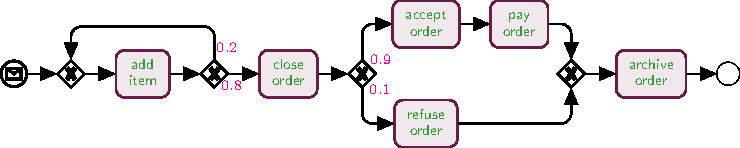
\includegraphics[width=\textwidth]{images/bpmn-order.pdf}
	\caption{BPMN model with choice probabilities capturing a simple order management process.}\label{fig:bpmn-order}
\end{figure}
\begin{figure}[!t]
	\centering
	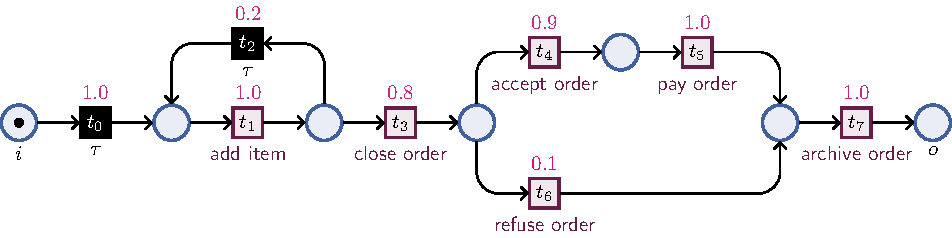
\includegraphics[width=\textwidth]{images/petri_order.pdf}
	\caption{Stochastic workflow net formalizing the BPMN diagram of Figure~\ref{fig:bpmn-order}.}\label{fig:petri_tut}
\end{figure}


\begin{figure}[!b]
	\centering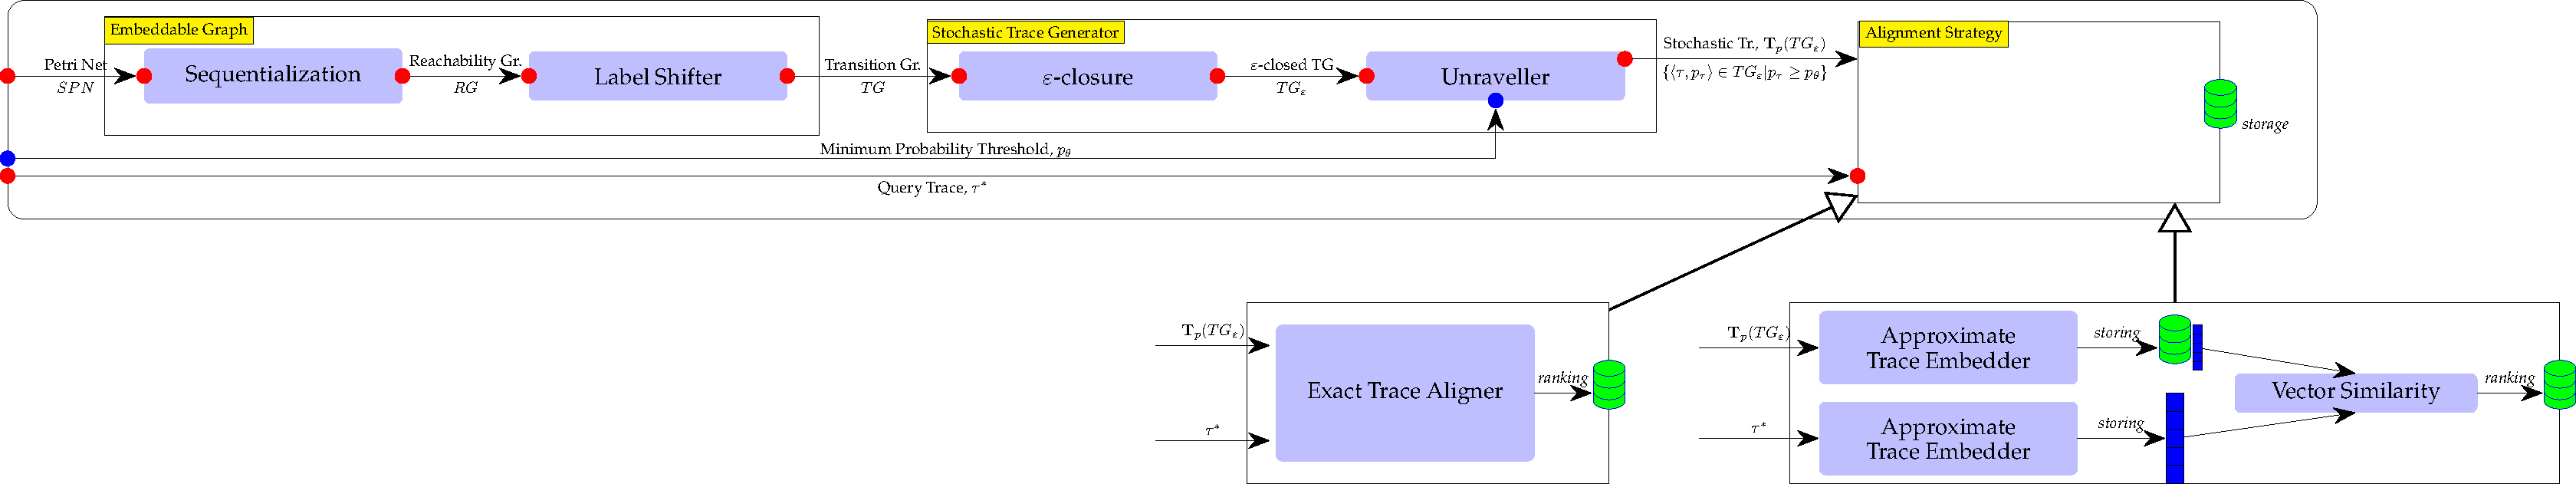
\includegraphics[width=\textwidth]{images/pipeline}
	\caption{Proposed pipeline to assess the probabilistic trace alignment.}\label{fig:pipe}
\end{figure}


%	
%%%%% Proposed part as the last part of the introduction:
%\texttt{\color{red}[TODO]}
%\todo{this is too specific for an introduction; in particular, too many details on how the experiments are done.}
%We implemented both strategies and perform experiments using a real life event log coming from a hospital system to empirically evaluate the properties of our proposed  strategy. Specifically, we (i) evaluate the correlation between the approximate rankings (using different ways for computing the embeddings) and the optimal ranking, and (ii)~compare the computation time for the exact trace alignment approach against the embedding-based approach. We show that the approximate ranking strategy exploiting a specific data structure (KD-Trees) provides the best trade-off between approximation and execution time, while being more efficient than both the exact ranking and the same approximate ranking with a different data structure (VP-Trees).
%In the next section, we describe the steps required by the tool to compute both alignment strategies. After briefly discussing some preliminary benchmarks, we propose some future work.